\documentclass[12pt]{article}
\usepackage[utf8]{inputenc}
\usepackage{times}
\usepackage{setspace}
\usepackage[space]{grffile}
\usepackage{latexsym}
\usepackage{textcomp}
\usepackage{longtable}
\usepackage{tabulary,threeparttable}
\usepackage{booktabs,array,multirow,siunitx}
\usepackage{amsfonts,amsmath,amssymb}
\usepackage[utf8]{inputenc}
\usepackage[english]{babel}
\usepackage[title]{appendix}
\usepackage{fancyhdr}
\usepackage{bbm}
\usepackage{afterpage}
\usepackage[margin=1in]{geometry}
\usepackage{threeparttable}
\usepackage{epsfig}
\usepackage{pdflscape}
\usepackage{natbib}
\usepackage{sectsty}
\subsectionfont{\normalfont\itshape}
\usepackage{setspace}
% \usepackage{endfloat}
\usepackage{graphicx}
\graphicspath{{./figs/}}
\usepackage{xr}

\externaldocument{main}
\begin{document}

\title{AJAE Appendix for ``The US Farm Credit System and Agricultural Development: Evidence from an Early Expansion, 1920-1940''}
\author{Jared Hutchins}
\date{}
\maketitle
\begin{center}
The material contained herein is supplementary to the article named in the title and published in the American Journal of Agricultural Economics.
\end{center}
\setcounter{table}{0}
\setcounter{figure}{0}
\renewcommand{\thetable}{\Alph{section}\arabic{table}}
\renewcommand{\thefigure}{\Alph{section}\arabic{figure}}
\doublespacing
\begin{appendices}
    \section{Covariate Effects}
    \label{appendix:covars}
    \setcounter{table}{0}
    \setcounter{figure}{0}
    
    The set of covariates for all the models consists of environmental characteristics, measures of the impact of the 1929 crisis on banks, and levels of federal government spending.
    Environmental controls include the only set of time-varying controls: average annual temperature and annual total rainfall.
    The squares of each of these measures are also included to control for the non-linearity of weather impacts.
    The remaining environmental controls are corn and wheat suitability from \citet{fao} and levels of erosion potential (percent of area at medium and high risk of erosion) from \citet{hornbeck_enduring_2012}.
    All of these measures are initially at the grid level but are averaged to the county level.
    To adjust for the impact of the 1929 crisis on bank closures in rural areas, another included covariate is the percent of deposits suspended in the period 1929 to 1933 \citep{fdic_1992}.
    Since PCAs may have been placed in areas with low banking, controlling for the pre-treatment level in bank access is important for identification.
    Finally, the aggregates of New Deal spending collected by \citet{fishback_can_2003} are included to control for the incidence of other programs other than PCAs.
    These data are only available as an aggregate, so the measure is technically time-invariant since it is the sum of spending for each county during the years 1933-1939.
    
    With the exception of temperature and rainfall, the controls are all time-invariant.
    In a TWFE model, time-invariant characteristics are collinear with fixed effects if they are not interacted with year fixed effects.
    While fixed effects controls for baseline differences that are time-invariant, we might worry that counties with different baseline characteristics, erosion for example, may experience different trends.
    Interacting these baseline characteristics with time fixed effects allows these time-invariant covariates to impact outcomes differently in different periods, similar to the way the state-by-year fixed effects allow each state to have its own unique time trend.
    
    Tables \ref{covar_temp}, \ref{covar_erosion}, and \ref{covar_govt} display the impact of the covariates on the studied outcomes.
    For most outcomes, temperature and rainfall are statistically significant and have non-linear effects.
    Corn and wheat soil suitability have varied impacts on outcomes, suggesting that trends likely are not significantly different across levels of soil suitability.
    Conversely, erosion has strong trend impacts.
    Erosion tends to be positively associated with many outcomes prior to 1930.
    With the onset of dust storms in 1935, erosion is negatively associated with many outcomes in 1935 and especially 1940.
    Suspended deposits do not have a statistically significant impact on outcomes with the exception of crop value per acre and tractors in 1940.
    
    Government spending is aggregated by \citet{fishback_can_2003} into four categories: relief, public works, grants, and loans. 
    Relief includes grants by administrations such as the Federal Emergency Relief Administration and the Civil Works Administration, public works includes spending by the Public Works Administration, and grants includes a variety of grant programs, one of which is the Agricultural Adjustment Act (AAA) payments meant to incentivize farmers to take land out of production to control price.
    The loans include a variety of different loans given by the federal government, including from the Farm Credit Administration.
    Note that since these spending outcomes happened during the period of the PCAs they are potentially endogenous controls. 
    If the activity of PCAs actually influenced the spending patterns of the federal government, New Deal spending would be an endogenous control. 
    As a compromise, New Deal grant programs and relief payments are included but not loan program spending, a program that is more likely to have been directly impacted by the presence of a PCA.
    
    As evidenced by the jump in predictive power when they are included (see Appendix B), these variables have significant prediction power for most of the outcomes.
    In particular, grants are negatively related to crop value before 1940 but positively after.
    This fits the narrative that many programs, much like PCAs, were targeted at areas that were worse off relative to other counties.
    
    \begin{table}[!htbp] \centering 
        \caption{Temperature and Soil Suitability} 
        \label{covar_temp} 
        \begin{threeparttable}[t]
        \footnotesize
      \begin{tabular}{@{\extracolsep{5pt}}lccccc} 
      \\[-1.8ex]\hline 
      \hline \\[-1.8ex] 
       & \multicolumn{5}{c}{\textit{Dependent Variable:}} \\ 
      \cline{2-6} 
      \\[-1.8ex] 
      &            &             &            &          &            \\
      & Corn Yield & Wheat Yield & Crop Value & Tractors & Fertilizer \\ 
      \hline \\[-1.8ex] 
    Temperature Avg     &  $-$1.199        & 0.059           & $-$0.905$^{**}$ & $-$0.237$^{***}$& $-$0.303$^{*}$ \\
                        &  (1.514)         & (0.579)         & (0.375)         & (0.067)         & (0.158)        \\
                        &                  &                 &                 &                 &                \\
    Temperature Avg Sqrd&  0.130           & $-$0.278$^{**}$ & 0.169$^{**}$    & 0.048$^{***}$   & 0.023          \\
                        &  (0.274)         & (0.121)         & (0.083)         & (0.015)         & (0.036)        \\
                        &                  &                 &                 &                 &                \\
    Rainfall Total          &  $-$0.793        & 1.112           & 2.714$^{***}$   & 0.791$^{***}$   & 1.129$^{**}$   \\
                        &  (0.988)         & (0.711)         & (0.771)         & (0.133)         & (0.447)        \\
                        &                  &                 &                 &                 &                \\
    Rainfall Total Sqrd     &  0.061           & $-$0.091$^{*}$  & $-$0.175$^{***}$& $-$0.060$^{***}$& $-$0.074$^{**}$\\
                        &  (0.067)         & (0.049)         & (0.052)         & (0.009)         & (0.031)        \\
    \quad               &                  &                 &                 &                 &                \\
                        &                 &                 &                   &                  & \\
    Corn Soil Suit.     &                 &                 &                   &                  & \\
    \quad 1920          & $-$0.063$^{***}$& 0.038$^{***}$   & 0.029$^{***}$   &                 & 0.006       \\
    \quad               & (0.024)         & (0.006)         & (0.010)         &                 & (0.007)     \\
    \quad               &                 &                 &                 &                 &             \\
    \quad 1925          & $-$0.006        & 0.030$^{***}$   & 0.047$^{***}$   & $-$0.003$^{**}$ & 0.005       \\
    \quad               & (0.027)         & (0.005)         & (0.009)         & (0.001)         & (0.004)     \\
    \quad               &                 &                 &                 &                 &             \\
    \quad 1935          & $-$0.088$^{***}$& $-$0.032$^{***}$&                 &                 &             \\
    \quad               & (0.026)         & (0.008)         &                 &                 &             \\
    \quad               &                 &                 &                 &                 &             \\
    \quad 1940          & $-$0.013        & $-$0.003        & 0.062$^{***}$   & 0.002           & $-$0.005    \\
    \quad               & (0.028)         & (0.011)         & (0.012)         & (0.002)         & (0.005)     \\
    \quad               &                 &                 &                 &                 &             \\
    Wheat Soil Suit.    &                 &                 &                   &                  &                  \\
    \quad 1920          & 0.088$^{***}$   & $-$0.052$^{**}$ & 0.115$^{***}$   &                 & 0.007                 \\
    \quad               & (0.032)         & (0.024)         & (0.038)         &                 & (0.030)               \\
    \quad               &                 &                 &                 &                 &                       \\
    \quad 1925          & 0.035           & $-$0.062$^{**}$ & 0.016           & 0.010$^{*}$     & 0.031                 \\
    \quad               & (0.044)         & (0.026)         & (0.036)         & (0.006)         & (0.020)               \\
    \quad               &                 &                 &                 &                 &                       \\
    \quad 1935          & 0.069           & 0.020           &                 &                 &                       \\
    \quad               & (0.045)         & (0.049)         &                 &                 &                       \\
    \quad               &                 &                 &                 &                 &                       \\
    \quad 1940          & 0.158$^{*}$     & 0.061           & $-$0.139$^{***}$& $-$0.017$^{***}$& $-$0.027$^{*}$        \\
    \quad               & (0.088)         & (0.052)         & (0.024)         & (0.004)         & (0.016)               \\
                        &                 &                 &                 &                 &                       \\
    \hline \\[-1.8ex] 
    Observations                       & 13,929          & 13,277          & 11,292          & 8,469           & 11,165          \\
    Adjusted R$^{2}$                   & 0.786           & 0.764           & 0.882           & 0.924           & 0.963           \\
    \hline 
    \hline \\[-1.8ex] 
    \end{tabular}
    \begin{tablenotes}
        \item {\footnotesize * \(p<0.10\), ** \(p<0.05\), *** \(p<0.01\).}
        \item {\footnotesize Standard errors clustered at the county-level.}
        \item {\footnotesize All specifications include county, year, and state-by-year fixed effects.}
        \end{tablenotes}
        \end{threeparttable} 
     
    \end{table} 
    
    \begin{table}[!htbp] \centering 
        \caption{Soil Erosion and Suspended Deposits} 
        \label{covar_erosion} 
        \begin{threeparttable}[t]
    
        \footnotesize
      \begin{tabular}{@{\extracolsep{5pt}}lccccc} 
      \\[-1.8ex]\hline 
      \hline \\[-1.8ex] 
      & \multicolumn{5}{c}{\textit{Dependent Variable:}} \\ 
      \cline{2-6} 
      \\[-1.8ex] 
      &            &             &            &          &            \\
      & Corn Yield & Wheat Yield & Crop Value & Tractors & Fertilizer \\ 
      \hline \\[-1.8ex] 
    Medium Erosion Pct        &                 &                 &                 &                 & \\
    \quad 1920                & $-$0.011        & 0.034           & 0.107$^{***}$   &                 & 0.034           \\
    \quad                     & (0.031)         & (0.035)         & (0.032)         &                 & (0.026)         \\
    \quad                     &                 &                 &                 &                 & \\
    \quad 1925                & 0.112$^{***}$   & $-$0.087$^{**}$ & 0.160$^{***}$   & 0.009$^{*}$     & $-$0.054$^{***}$\\
    \quad                     & (0.041)         & (0.038)         & (0.037)         & (0.005)         & (0.018)         \\
    \quad                     &                 &                 &                 &                 & \\
    \quad 1935                & $-$0.116$^{***}$& 0.168$^{***}$   &                 &                 & \\
    \quad                     & (0.044)         & (0.051)         &                 &                 & \\
    \quad                     &                 &                 &                 &                 & \\
    \quad 1940                & $-$0.081$^{*}$  & 0.064           & $-$0.230$^{***}$& $-$0.006        & $-$0.135$^{***}$\\
                              & (0.044)         & (0.047)         & (0.041)         & (0.006)         & (0.023)         \\
                              &                 &                 &                 &                 & \\
    High Erosion Pct          &                 &                 &                 &                 & \\
    \quad 1920                & $-$0.0004       & $-$0.029        & 0.189$^{***}$   &                 & 0.059$^{**}$    \\
    \quad                     & (0.032)         & (0.041)         & (0.031)         &                 & (0.030)         \\
    \quad                     &                 &                 &                 &                 & \\
    \quad 1925                & 0.245$^{***}$   & $-$0.107$^{***}$& 0.117$^{***}$   & 0.034$^{***}$   & $-$0.025        \\
    \quad                     & (0.046)         & (0.040)         & (0.032)         & (0.005)         & (0.020)         \\
    \quad                     &                 &                 &                 &                 & \\
    \quad 1935                & $-$0.232$^{***}$& 0.221$^{***}$   &                 &                 & \\
    \quad                     & (0.048)         & (0.061)         &                 &                 & \\
    \quad                     &                 &                 &                 &                 & \\
    \quad 1940                & 0.045           & 0.068           & $-$0.292$^{***}$& $-$0.018$^{***}$& $-$0.182$^{***}$\\
                              & (0.054)         & (0.055)         & (0.052)         & (0.006)         & (0.024)         \\
                              &                 &                 &                 &                 & \\
     Suspended Deposits       &                 &                 &                 &                 & \\
    \quad 1920                & 0.072           & $-$0.021        & $-$0.038        &                 & $-$0.023      \\
    \quad                     & (0.080)         & (0.090)         & (0.066)         &                 & (0.063)       \\
    \quad                     &                 &                 &                 &                 & \\
    \quad 1925                & $-$0.131        & 0.110           & 0.001           & $-$0.012        & $-$0.025      \\
    \quad                     & (0.110)         & (0.087)         & (0.070)         & (0.009)         & (0.043)       \\
    \quad                     &                 &                 &                 &                 & \\
    \quad 1935                & 0.010           & $-$0.092        &                 &                 & \\
    \quad                     & (0.104)         & (0.117)         &                 &                 & \\
    \quad                     &                 &                 &                 &                 & \\
    \quad 1940                & $-$0.115        & 0.004           & $-$0.167$^{*}$  & 0.023$^{**}$    & $-$0.072      \\
                              & (0.109)         & (0.100)         & (0.090)         & (0.011)         & (0.047)       \\
                              &                 &                 &                 &                 & \\
    \hline \\[-1.8ex] 
    Observations                       & 13,929          & 13,277          & 11,292          & 8,469           & 11,165          \\
    Adjusted R$^{2}$                   & 0.786           & 0.764           & 0.882           & 0.924           & 0.963           \\
    \hline 
    \hline \\[-1.8ex] 
    \end{tabular} 
    \begin{tablenotes}
        \item {\footnotesize * \(p<0.10\), ** \(p<0.05\), *** \(p<0.01\).}
        \item {\footnotesize Standard errors clustered at the county-level.}
        \item {\footnotesize All specifications include county, year, and state-by-year fixed effects.}
        \end{tablenotes}
        \end{threeparttable} 
    
    \end{table} 
    
    
    \begin{table}[!htbp] \centering 
        \caption{Government Payments and Aid} 
        \label{covar_govt} 
        \begin{threeparttable}[t]
    
        \footnotesize
      \begin{tabular}{@{\extracolsep{5pt}}lccccc} 
      \\[-1.8ex]\hline 
      \hline \\[-1.8ex] 
      & \multicolumn{5}{c}{\textit{Dependent Variable:}} \\ 
      \cline{2-6} 
      \\[-1.8ex] 
      &            &             &            &          &            \\
      & Corn Yield & Wheat Yield & Crop Value & Tractors & Fertilizer \\ 
      \hline \\[-1.8ex]
    Total Relief                &               &                 &                &                 &           \\
    \quad 1920                      & $-$0.035        & 0.128$^{***}$   & 0.089$^{***}$   &                 & $-$0.008       \\
    \quad                           & (0.028)         & (0.019)         & (0.022)         &                 & (0.014)        \\
    \quad                           &                 &                 &                 &                 &                \\
    \quad 1925                      & $-$0.020        & 0.094$^{***}$   & $-$0.019        & 0.065$^{***}$   & $-$0.025$^{**}$\\
    \quad                           & (0.033)         & (0.020)         & (0.021)         & (0.005)         & (0.010)        \\
    \quad                           &                 &                 &                 &                 &                \\
    \quad 1935                      & $-$0.054        & 0.079$^{***}$   &                 &                 &                \\
    \quad                           & (0.037)         & (0.029)         &                 &                 &                \\
    \quad                           &                 &                 &                 &                 &                \\
    \quad 1940                      & 0.094$^{**}$    & 0.047$^{*}$     & $-$0.213$^{***}$& $-$0.047$^{***}$& $-$0.023$^{*}$ \\
                                    & (0.037)         & (0.025)         & (0.028)         & (0.005)         & (0.012)        \\
                                    &                 &                 &                 &                 &                \\
    Total Public Works                  &               &                 &                &                 &                  \\
    \quad 1920                      & $-$0.013        & 0.037$^{***}$   & 0.045$^{***}$   &                 & $-$0.005         \\
    \quad                           & (0.011)         & (0.009)         & (0.012)         &                 & (0.007)          \\
    \quad                           &                 &                 &                 &                 &                  \\
    \quad 1925                      & 0.012           & 0.029$^{***}$   & 0.025$^{**}$    & 0.013$^{***}$   & $-$0.005         \\
    \quad                           & (0.014)         & (0.008)         & (0.011)         & (0.003)         & (0.005)          \\
    \quad                           &                 &                 &                 &                 &                  \\
    \quad 1935                      & 0.042$^{**}$    & 0.033$^{**}$    &                 &                 &                  \\
    \quad                           & (0.020)         & (0.013)         &                 &                 &                  \\
    \quad                           &                 &                 &                 &                 &                  \\
    \quad 1940                      & 0.089$^{***}$   & 0.009           & $-$0.027$^{*}$  & $-$0.005$^{**}$ & $-$0.006         \\
                                    & (0.020)         & (0.011)         & (0.015)         & (0.002)         & (0.006)          \\
                                    &                 &                 &                 &                 &                  \\
    Total Grants                   &               &                 &                &                 &                  \\
    \quad 1920                      & 0.029           & $-$0.201$^{***}$& $-$0.251$^{***}$&                 & $-$0.049$^{**}$ \\
    \quad                           & (0.039)         & (0.028)         & (0.035)         &                 & (0.019)         \\
    \quad                           &                 &                 &                 &                 &                 \\
    \quad 1925                      & 0.070           & $-$0.139$^{***}$& $-$0.145$^{***}$& $-$0.093$^{***}$& 0.002           \\
    \quad                           & (0.048)         & (0.028)         & (0.034)         & (0.007)         & (0.014)         \\
    \quad                           &                 &                 &                 &                 &                 \\
    \quad 1935                      & $-$0.044        & $-$0.120$^{***}$&                 &                 &                 \\
    \quad                           & (0.052)         & (0.040)         &                 &                 &                 \\
    \quad                           &                 &                 &                 &                 &                 \\
    \quad 1940                      & $-$0.107$^{**}$ & $-$0.015        & 0.367$^{***}$   & 0.056$^{***}$   & $-$0.006        \\
                                    & (0.054)         & (0.036)         & (0.040)         & (0.007)         & (0.018)         \\
                                    &                 &                 &                 &                 &                 \\
    
    \hline \\[-1.8ex] 
    Observations                       & 13,929          & 13,277          & 11,292          & 8,469           & 11,165          \\
    Adjusted R$^{2}$                   & 0.786           & 0.764           & 0.882           & 0.924           & 0.963           \\
    \hline 
    \hline \\[-1.8ex] 
    \end{tabular} 
    \begin{tablenotes}
        \item {\footnotesize * \(p<0.10\), ** \(p<0.05\), *** \(p<0.01\).}
        \item {\footnotesize Standard errors clustered at the county-level.}
        \item {\footnotesize All specifications include county, year, and state-by-year fixed effects.}
        \end{tablenotes}
        \end{threeparttable} 
    
    \end{table} 

\section{Covariates and Overfitting}
\label{appendix:overfit}
Including too many covariates in a regression can often lead to overfitting the data.
This becomes a problem in causal inference when too much identifying variation is ``purged'' from the data, making the estimation of causal parameters like the ATT very difficult.
In this case, the inclusion of state fixed effects interacted with time and other time-invariant factors interacted with time could purge variation we would want to use to identify the effects of PCAs.
In this section, I use cross-validation to examine the impacts of including more and more controls into the regression on the prediction error of the model.
A model that is overfitting should decline in terms of prediction error as more controls are included.

I examine three outcomes which had a relationship to PCA placement: corn yield, crop value per acre, and tractors per farm.
I use 10-fold cross validation, which randomly splits the data into ten equally sized segments, trains the model on nine of those segments, and predicts the outcome on the remaining segment.
I measure the root mean squared error (RMSE) for each of these ten predictions and then average them across all ten.
I then repeat this process 100 times to ensure robustness to where the splits happen each time.
There are six levels of covariates that are added gradually across the models: two way fixed effects, state-by-year fixed effects, environmental variables, weather variables, AAA payments, and all New Deal spending.

\begin{figure}
\caption{RMSEs Across Covariates}
\label{rmses}
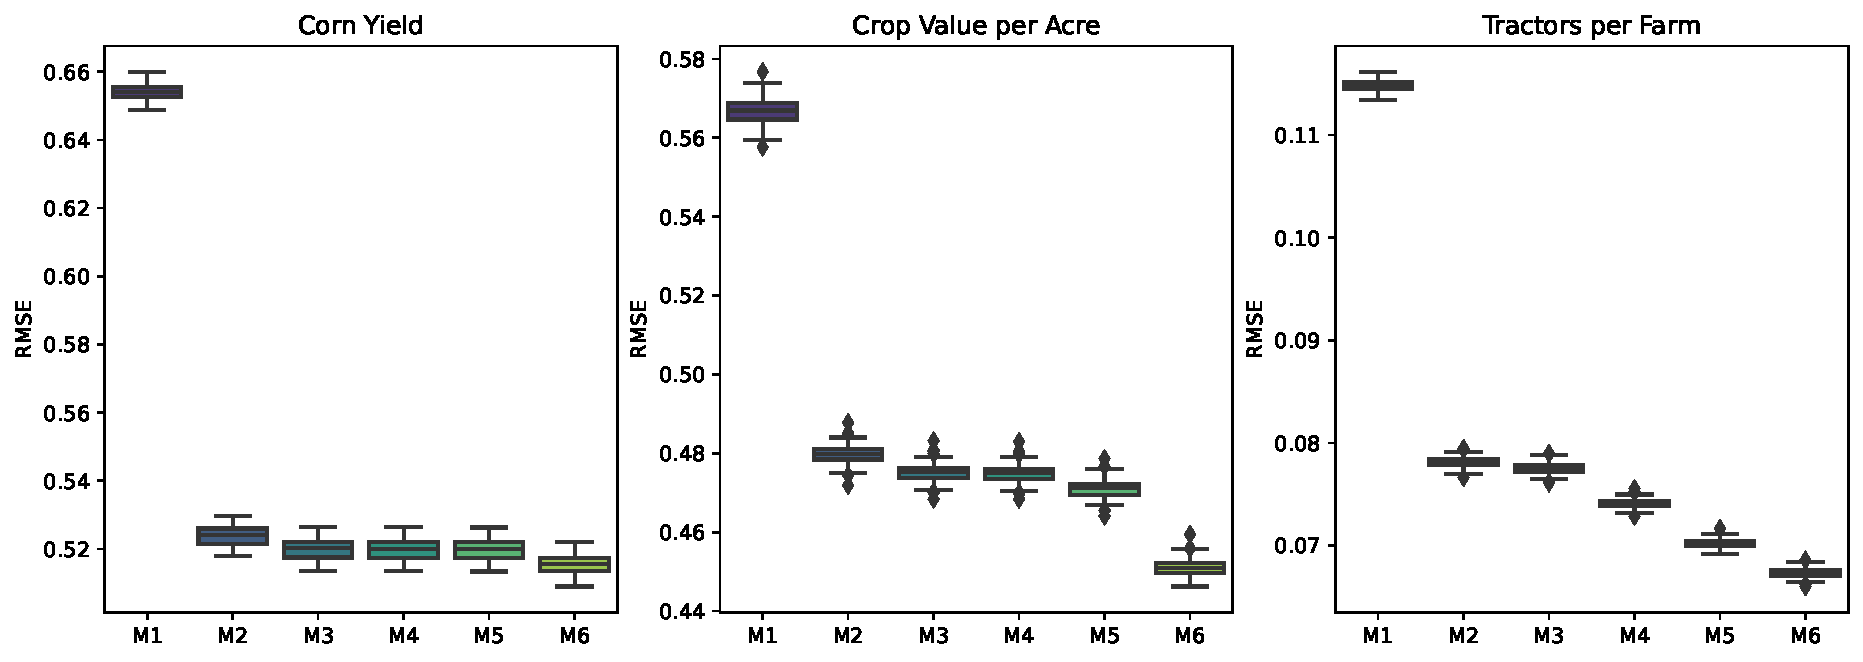
\includegraphics[width=\textwidth]{Model_RMSEs.pdf}
\centering
\begin{tabular}{cl}
Model Number & Added controls \\ \hline 
1  & County and year fixed effects.\\
2  & State-by-year fixed effects. \\
3  & Environmental variables (soil suitability, erosion), Bank deposits lost. \\
4  & Weather variables (average temperature and annual precipitation). \\
5  & AAA payments. \\
6  & All New Deal spending.     
\end{tabular}
\end{figure}

Figure \ref{rmses} shows the RMSEs for all 100 iterations of the procedure across levels of controls in a box-whisker plot.
For all three outcomes, RMSE is at least non-monotonically decreasing in the level of controls.
Adding state-by-year fixed effects (M1 to M2) causes the largest decrease in RMSE for all three models. 
Tractors per farm in particular shows a decrease in RMSE with each level of control added.
For corn yield and crop value per acre, there is a small decrease in RMSE after environmental variables are added (M2 to M3) and a decrease in RMSE when all New Deal spending variables are used.
Cross-validation confirms that adding all of the covariates to the regression does not lead to overfitting in these outcomes and is likely not purging any useful variation from the data needed to identify the ATT.
\setcounter{table}{0}
\setcounter{figure}{0}
\renewcommand{\thetable}{\Alph{section}\arabic{table}}


\section{Robustness Checks}
\subsection{Binary Definition of Treatment}
\label{appendix_binary}

A helpful baseline comparison to the estimates using a continuous variable or a discretized analog is the simple binary treatment model.
Much more is known about the properties of this model than difference-in-difference estimators using continuous variables.
The most straightforward ``binary treatment'' definition in the case of the PCAs would be whether the PCA is located in the county boundaries (regardless of distance from the centroid).
In this section, I present the results of the analysis using this treatment definition as well as some alternatives to check robustness.

\begin{figure}
    \caption{Binary Treatment Definitions}
    \label{binary_def}
    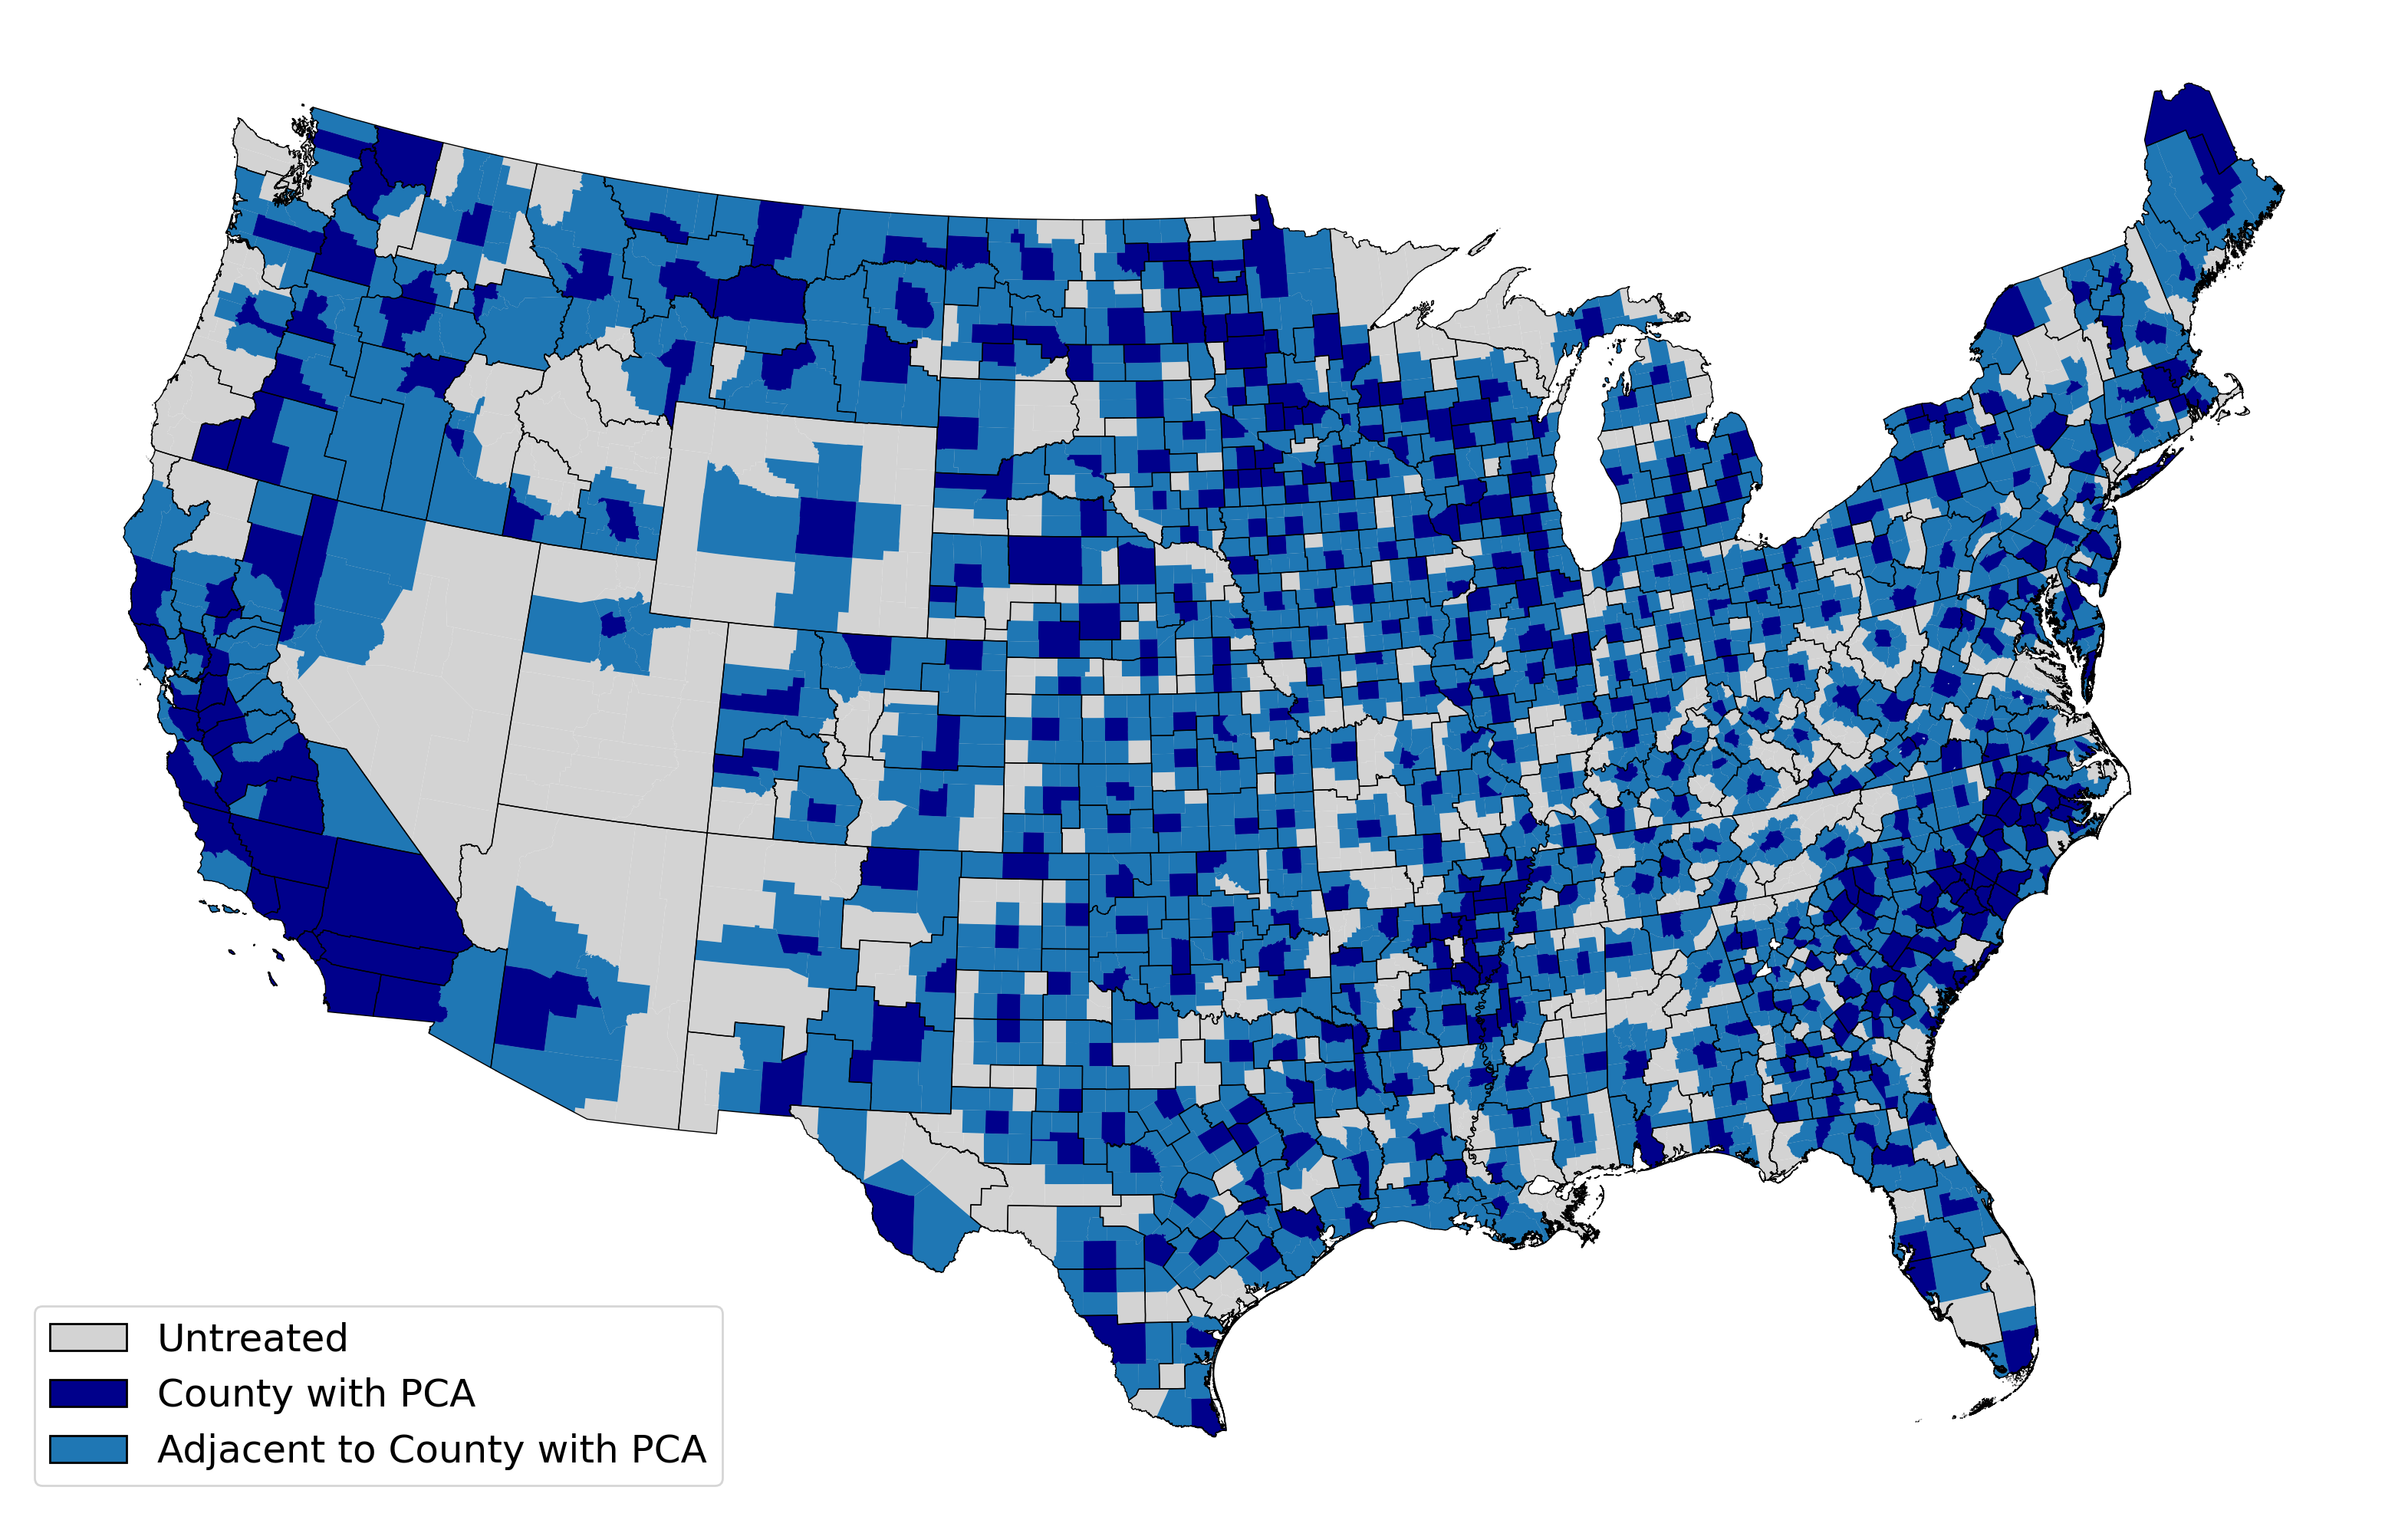
\includegraphics[width=\textwidth]{binary_map.png}
    \centering
    \begin{tabular}{lccccc}
         & \multicolumn{5}{c}{Distance to PCA (km)} \\
        {} &  (0, 30] &  (30, 45] &  (45, 60] &  (60, 100] &  $>$ 100 \\ \hline
        Untreated    &     0.24 &      4.31 &     13.77 &      49.46 &    32.22 \\
        County with PCA            &    91.98 &      5.22 &      1.49 &       0.56 &     0.75 \\
        Adjacent to County With PCA &    14.06 &     41.65 &     23.76 &      17.30 &     3.23 \\
        \hline \hline
        \multicolumn{2}{l}{\footnotesize{Each number is the percent of the row sum.}} 
    \end{tabular}
    
    \end{figure}
    
Figure \ref{binary_def} shows two definitions of treatment and how they relate to the binned distance measure of treatment.
The darkest counties in the figure are counties which have a PCA anywhere within their boundaries.
The lighter, colored counties are counties that border counties with PCAs within their coverage area.
Counties that border PCA counties but are outside the coverage are not considered adjacent counties, for example.
Counties that do not contain PCAs or are not adjacent to one (``Untreated'') are nearly all more than 60 kilometers away from their serving PCA (about 82\% of counties).
Counties with a PCA are almost entirely within 30 kilometers of their PCA (about 92\% of counties), and counties adjacent to PCAs are mostly within the 30-60 kilometer range (though about 30\% are in the 0-30 and 60-100 ranges).
Testing whether counties with PCAs have different outcomes than other counties essentially amounts to testing whether counties within 30 km of a PCA are different than every other county.
It imposes the restriction that counties without PCAs cannot benefit from the placement of a PCA.

Table \ref{pca_binary} shows the results of the estimation when the measure of treatment is simply whether a PCA is in the county ($PCA =1 $) or not ($PCA=0$).
Very few coefficients are statistically significant with the exception of the post-treatment effects for crop value and tractors.
Those estimates imply that counties with PCAs had five percent higher crop value per acre and 1.1\% more tractors per farm.
The other significant coefficients suggest that areas with PCAs had lower corn and wheat yield and a lower number of tractors prior to PCA placement.
These results demonstrate that the highly significant results found in the main specifications are mostly driven by comparing areas with PCAs to farther areas.
Since counties within 45 km of a PCA tend to be the same in terms of crop value per acre, comparing counties within 30 km to every other county results in a difference that is only weakly statistically different.

Table \ref{pca_binary_adj} tests two more specifications for crop value per acre: one where all counties adjacent to PCA counties are considered treated (all shaded areas in Figure \ref{binary_def}), and one where only PCA counties are treated and all non-adjacent counties are dropped (the unshaded areas in Figure \ref{binary_def} are dropped from the sample).
When all counties adjacent to PCAs are considered treated, the effect increases to 6.7\%. 
In this specification, counties within 60 km of a PCA are essentially being compared to counties farther than 60 km.
The third column drops the ``Untreated'' counties and tests whether counties with PCAs are statistically different than counties that are adjacent.
The result is that the difference is no longer statistically different.

Much like the main results, these results demonstrate that PCAs did not solely benefit the county they were located in. 
The benefits spilled over into at least the adjacent counties, though not beyond this radius.
As \citet{Arnold1958} pointed out, farmers in farther counties likely did not know about the existence of PCAs.
The analysis here seems to suggest that ``farther counties'' were likely more than 60 km away, as differences are only apparent comparing counties within 60 to farther than 60.


\def\sym#1{\ifmmode^{#1}\else\(^{#1}\)\fi}

\begin{table}[!htbp] \centering 
    \caption{PCA Binary Definition} 
    \label{pca_binary} 

    Base category: Year $=$ 1930

    \begin{threeparttable}[t]
\footnotesize   

  \begin{tabular}{@{\extracolsep{5pt}}lccccc} 
  \\[-1.8ex]\hline 
  \hline \\[-1.8ex] 
   & \multicolumn{5}{c}{\textit{Dependent Variable:}} \\ 
  \cline{2-6} 
  \\[-1.8ex] & Corn Yield & Wheat Yield & Crop Value & Tractors & Fertilizer \\ 
  \hline \\[-1.8ex] 
PCA $\times$ 1920 & $-$0.036$^{*}$ & $-$0.049$^{**}$ & $-$0.012 &  & $-$0.006 \\ 
& (0.020) & (0.019) & (0.021) &  & (0.017) \\ 
& & & & & \\ 
PCA $\times$ 1925 & 0.017 & $-$0.023 & 0.033 & $-$0.005$^{*}$ & 0.004 \\ 
& (0.026) & (0.019) & (0.027) & (0.003) & (0.013) \\ 
& & & & & \\ 
PCA $\times$ 1935 & 0.051 & 0.029 &  &  &  \\ 
& (0.032) & (0.033) &  &  &  \\ 
& & & & & \\ 
PCA $\times$ 1940 & 0.047 & 0.014 & 0.050$^{*}$ & 0.011$^{***}$ & 0.009 \\ 
& (0.032) & (0.028) & (0.028) & (0.004) & (0.015) \\ 
& & & & & \\ 
\hline \\[-1.8ex] 
Observations & 13,929 & 13,277 & 11,292 & 8,469 & 11,165 \\ 
Adjusted R$^{2}$ & 0.786 & 0.765 & 0.881 & 0.926 & 0.963 \\ 
\hline 
\hline \\[-1.8ex] 
\end{tabular} 
\begin{tablenotes}
    \item {\footnotesize * \(p<0.10\), ** \(p<0.05\), *** \(p<0.01\).}
    \item {\footnotesize Standard errors clustered at the county-level.}
    \item {\footnotesize All specifications include county, year, and state-by-year fixed effects.}
    \end{tablenotes}
    \end{threeparttable} 

\end{table}










\begin{table}[!htbp] \centering 
    \caption{Alternative PCA Binary Definition} 
    \label{pca_binary_adj} 

    Base category: Year $=$ 1930

    \begin{threeparttable}[t]
\footnotesize   
\begin{tabular}{@{\extracolsep{5pt}}lccc} 
    \\[-1.8ex]\hline 
    \hline \\[-1.8ex] 
     & \multicolumn{3}{c}{Crop Value per Acre} \\ 
    \cline{2-4} 
    \\[-1.8ex] &  & &  \\ 
    \\[-1.8ex] & County with PCA & Adjacent to     & County with PCA\\ 
               &                 & County with PCA & Adjacent Only \\
    \hline \\[-1.8ex] 
    
    PCA $\times$ 1920         & $-$0.012              & 0.013       & $-$0.010          \\
                              & (0.021)               & (0.020)     & (0.022)           \\
                              &                       &             &                   \\
    PCA $\times$ 1925         & 0.033                 & 0.029       & 0.033             \\
                              & (0.027)               & (0.024)     & (0.026)           \\
                              &                       &             &                   \\
    PCA $\times$ 1940         & 0.050$^{*}$           & 0.067$^{**}$& 0.040             \\
                              & (0.028)               & (0.028)     & (0.029)           \\
                              &            &             &          \\
    \hline \\[-1.8ex] 
    
    Observations & 11,292 & 11,292 & 8,352 \\ 
    Adjusted R$^{2}$ & 0.881 & 0.881 & 0.881 \\ 
    \hline 
    \hline \\[-1.8ex] 

\end{tabular} 


    \begin{tablenotes}
        \item {\footnotesize * \(p<0.10\), ** \(p<0.05\), *** \(p<0.01\).}
        \item {\footnotesize Standard errors clustered at the county-level.}
        \item {\footnotesize All specifications include county, year, and state-by-year fixed effects.}
        \end{tablenotes}
        \end{threeparttable} 
    
    \end{table}
    








\subsection{Alternative Standard Errors}
\label{alt_se}
The main results use standard errors that are clustered by county.
As a robustness check, I estimate the binned distance model using standard errors that are robust to spatial correlation.
If counties are cross-sectionally interdependent in terms of outcomes, its important to take into account that errors from one county are correlated to its neighbors.
The standard error method laid out in \citet{conley1999gmm} is often referred to as ``Conley standard errors'' and are routinely applied in this case.

Table \ref{conley_se} shows the coefficients for the post-estimation period, 1940, for all the outcomes with county clustered standard errors and Conley standard errors.
In general, the Conley standard errors are not meaningfully different than the county clustered errors.
They are both bigger and smaller than the county clustered errors for different coefficients.
The pattern of significance is overall unchanged, with the exception of the tractors coefficient for 30-45 km from a PCA.
Using Conley standard errors, the standard error is twice as large which implies that counties 30-45 km from a PCA are not statistically different than those within 30 km of a PCA.
This is more consistent with the pattern of crop value per acre and corn yield: counties within 60 km of a PCA are usually similar in terms of outcomes, whereas counties beyond 60 km are much different in terms of outcomes.








\begin{table}
    \centering

    \caption{Conley Standard Errors}
    1940 Coefficients Only
    \label{conley_se}
\footnotesize   
\vspace{.5cm} 
% Negative coefficients indicate a positive association \\
% between PCA proximity and agricultural outcomes.\\

Base category: Year $=$ 1930 and $<$ 30 km from a PCA
    \begin{threeparttable}[t]
    \footnotesize


\begin{tabular}{lcccccc}
\hline\hline
% & \multicolumn{6}{c}{} \\
& \multicolumn{6}{c}{\textbf{Crop Yield}} \\
[.5em]
&\multicolumn{2}{c}{IHS(Corn Yield)}&\multicolumn{2}{c}{IHS(Wheat Yield)}&\multicolumn{2}{c}{IHS(Crop Value per Acre)}\\
[.5em]
\cline{2-7}
& & & & & & \\ 
Distance  & County           & Conley SE & County        & Conley SE &County        & Conley SE   \\
              & Clustered SE     &           &  Clustered SE &           & Clustered SE &              \\ \hline 
$[30, 45)$ km & $-$0.032       & $-$0.032        & $-$0.014   & $-$0.014    & $-$0.024        & $-$0.024           \\
              & (0.030)        & (0.020)         & (0.030)    & (0.055)     & (0.028)         & (0.043)            \\
              &                &                 &            &             &                 &                    \\
$[45, 60)$ km & $-$0.011       & $-$0.011        & 0.011      & 0.011       & $-$0.075$^{**}$ & $-$0.075$^{***}$   \\
              & (0.035)        & (0.027)         & (0.033)    & (0.019)     & (0.034)         & (0.027)            \\
              &                &                 &            &             &                 &                    \\
$[60, 100)$ km& $-$0.093$^{**}$& $-$0.093$^{***}$& $-$0.007   & $-$0.007    & $-$0.157$^{***}$& $-$0.157$^{***}$   \\
              & (0.039)        & (0.030)         & (0.032)    & (0.025)     & (0.035)         & (0.025)            \\
              &                &                 &            &             &                 &                    \\
$>$ 100 km    & $-$0.148$^{**}$& $-$0.148$^{**}$ & 0.061      & 0.061$^{**}$& $-$0.200$^{***}$& $-$0.200$^{***}$   \\
              & (0.072)        & (0.062)         & (0.051)    & (0.029)     & (0.054)         & (0.031)            \\
         [1em]
         \hline
         Obs      &   \multicolumn{2}{c}{13,929}  &   \multicolumn{2}{c}{13,277} &   \multicolumn{2}{c}{11,292} \\
         Adj. $R^2$ &  \multicolumn{2}{c}{0.786} &\multicolumn{2}{c}{0.765}      &  \multicolumn{2}{c}{0.882}   \\

\hline\hline
% & \multicolumn{6}{c}{} \\
 & \multicolumn{4}{c}{\textbf{Inputs}} & & \\
[.5em]

&\multicolumn{2}{c}{IHS(\# Tractors/Farm)} &   \multicolumn{2}{c}{IHS(\$ Fert/Acre)} & & \\
[.5em]
\cline{2-7} 
& & & & & & \\
Distance & County           & Conley SE & County        & Conley SE & &  \\
              & Clustered SE     &           &  Clustered SE &           & &   \\ 
\hline
$[30, 45)$ km & $-$0.009$^{**}$ & $-$0.009        & $-$0.002 & $-$0.002   & &   \\
              & (0.004)         & (0.008)         & (0.014)  & (0.022)    & &   \\
              &                 &                 &          &            & &   \\
$[45, 60)$ km & $-$0.010$^{**}$ & $-$0.010$^{***}$& $-$0.014 & $-$0.014   & &   \\
              & (0.004)         & (0.003)         & (0.017)  & (0.017)    & &   \\
              &                 &                 &          &            & &   \\
$[60, 100)$ km& $-$0.020$^{***}$& $-$0.020$^{***}$& $-$0.005 & $-$0.005   & &   \\
              & (0.004)         & (0.003)         & (0.016)  & (0.012)    & &   \\
              &                 &                 &          &            & &   \\
$>$ 100 km    & $-$0.040$^{***}$& $-$0.040$^{***}$& $-$0.0002& $-$0.0002  & &   \\
              & (0.007)         & (0.005)         & (0.031)  & (0.019)    & &   \\
      [1em] \hline 
      Obs      &    \multicolumn{2}{c}{8,469} & \multicolumn{2}{c}{11,165} & & \\
      Adj. $R^2$ &  \multicolumn{2}{c}{0.926} & \multicolumn{2}{c}{0.963}  & & \\\hline 
    \hline 
\end{tabular}
\begin{tablenotes}
    \item {\footnotesize The coefficients displayed are \textit{not} transformed using \citet{bellemare_elasticities_2020}.}
    \item {\footnotesize * \(p<0.10\), ** \(p<0.05\), *** \(p<0.01\).}
    \item {\footnotesize All specifications include county, year, and state-by-year fixed effects.}
    \end{tablenotes}
\end{threeparttable}
\end{table}

\subsection{Regional PCA Effects}
\label{appendix:regional}
In this section, I test whether PCAs had different effects in the Great Plains compared to rest of the county east of the Great Plains (``East and Midwest'').
The East and Midwest are used as a comparison group since it is more similar to the Great Plains than the area west of the Great Plains.
Since the Great Plains were affected by dust storms in the 1930s, this robustness check helps us understand how PCAs may have operated differently due to the environmental shocks present in that region.
Omitting the Western US from the model is also helpful given how most of the West depends less on crop agriculture and more on livestock.
In what follows, I used the definition of the Great Plains used in \citet{hornbeck_enduring_2012} which is the same as in Figure \ref{sample_map}.

Table \ref{gp_table} shows corn yield, crop value per acre, and tractor usage across the Great Plains and the East and Midwest.
It is immediately clear that corn yields were strongest in the Great Plains, an area which contains some states that would become part of the ``Corn Belt.''
The effects for crop value per acre are strongest for the East and Midwest, though still somewhat siginificant for the Great Plains.
Tractor usage is significant in both areas, though PCAS are associated with at most seven percent more tractor usage in the Great Plains.
This is much less than the one to four percent found in the main specification.
Since the Great Plains had larger farms and more extensive planting, it seems plausible that the PCAs would influence tractor usage most in the Great Plains.
To summarize, this exercise shows us that crop value per acre gains are strongest in the East and Midwest, whereas corn yield and tractor usage gains are strongest in the Great Plains.





\begin{table}
    \caption{Regional PCA Effects}
    \label{gp_table}
    \centering
    \begin{threeparttable}[t]
        \footnotesize

\begin{tabular}{lcccc}
    \hline\hline
& \multicolumn{4}{c}{Corn Yield} \\
\cline{2-5} \\ 
& \multicolumn{2}{c}{East and Midwest} & \multicolumn{2}{c}{Great Plains} \\
Distance from PCA& 1935          & 1940         & 1935           & 1940            \\ \hline
$(30, 45]$ km    & $-$0.014      & $-$0.034     & $-$0.146$^{**}$& 0.006           \\
                 & (0.022)       & (0.032)      & (0.057)        & (0.063)         \\
                 &               &              &                &                 \\
$(45, 60]$ km    & $-$0.005      & 0.029        & $-$0.096       & 0.006           \\
                 & (0.027)       & (0.038)      & (0.064)        & (0.068)         \\
                 &               &              &                &                 \\
$(60, 100]$ km   & $-$0.044$^{*}$& $-$0.020     & $-$0.122$^{**}$& $-$0.084        \\
                 & (0.026)       & (0.037)      & (0.061)        & (0.065)         \\
                 &               &              &                &                 \\
$>$ 100 km       & $-$0.111      & 0.012        & $-$0.201$^{**}$& $-$0.207$^{**}$ \\
                 & (0.075)       & (0.082)      & (0.093)        & (0.093)         \\
                 &               &              &                &                 \\ \hline \\[-1.8ex]
Observations          & \multicolumn{2}{c}{8,591}  & \multicolumn{2}{c}{4,334} \\
Adjusted R$^{2}$      & \multicolumn{2}{c}{0.832}  & \multicolumn{2}{c}{0.793} \\
Pre-Trend F-Statistic & \multicolumn{2}{c}{0.452}  & \multicolumn{2}{c}{0.39 } \\
Pre-Trend p-value     & \multicolumn{2}{c}{0.89 }  & \multicolumn{2}{c}{0.926} \\ 
\hline\hline

& \multicolumn{2}{c}{Crop Value}   & \multicolumn{2}{c}{Tractors}      \\
                 \cline{2-5} \\ 
                 & East and Midwest& Great Plains   & East and Midwest& Great Plains    \\
Distance from PCA& 1940            & 1940           & 1940            & 1940  \\ \hline
$(30, 45]$ km    & $-$0.010        & $-$0.042       & $-$0.005        & $-$0.016$^{*}$  \\
                 & (0.031)         & (0.056)        & (0.003)         & (0.010)         \\
                 &                 &                &                 & \\
$(45, 60]$ km    & $-$0.082$^{**}$ & $-$0.027       & $-$0.006$^{*}$  & $-$0.021$^{**}$ \\
                 & (0.035)         & (0.063)        & (0.003)         & (0.010)         \\
                 &                 &                &                 & \\
$(60, 100]$ km   & $-$0.114$^{***}$& $-$0.127$^{**}$& $-$0.011$^{***}$& $-$0.035$^{***}$\\
                 & (0.036)         & (0.055)        & (0.003)         & (0.010)         \\
                 &                 &                &                 & \\
$>$ 100 km       & $-$0.249$^{***}$& 0.051          & $-$0.012$^{**}$ & $-$0.069$^{***}$\\
                 & (0.060)         & (0.090)        & (0.006)         & (0.014)         \\
                 &                 &                &                 & \\\hline \\[-1.8ex]
  Observations                      &  6,880          &  3,520         & 5,160           &  2,640          \\
  Adjusted R$^{2}$                  &  0.869          &  0.886         & 0.945           &  0.913          \\
  Pre-Trend F-Statistic             &  0.689          &  0.816         & 0.57            &  0.653          \\
  Pre-Trend p-value                 &  0.702          &  0.588         & 0.684           &  0.625          \\ \hline 
  \hline 
\end{tabular}

  \begin{tablenotes}
    \item {\footnotesize * \(p<0.10\), ** \(p<0.05\), *** \(p<0.01\).}
    \item {\footnotesize All specifications include county, year, and state-by-year fixed effects.}
  \end{tablenotes}
\end{threeparttable}
\end{table}

\subsection{Hyrbid Corn Adoption}
\label{appendix:hybrid}
A major innovation that influenced corn yields starting in 1933 is hybrid corn.
It is a frequent topic of study given how quickly the use of hybrid corn diffused to corn producers; hardly any farms had planted it in 1926, whereas by 1941 nearly ever corn farmer used hybrid seed \citep{griliches1960hybrid,ryan1950acceptance}.
PCAs provided production credit which may have sped up adoption of hybrid corn since production credit was well suited to buying variable inputs like seed.
This may halp explain why we see the PCAs having an effect on corn yield in the main model, as hybrid corn varieties are particularly resilient to drought.
While county-level adoption data is not widely available, there is state adoption level data on the percentage of acres planted to hybrid corn available in \citet{nass_agricultural_1945}.

In this robustness check, I examine whether counties in ``early adopter'' states in 1935 experienced different PCA effects with regards to corn yield.
I contrast this to ``late adopter'' states which did not plant hybrid corn until 1940. 
Figure \ref{corn_map} shows which states had planted hyrbid corn in 1935 and which had planted in 1940.
To be consistent with the hypothesis that PCAs facilitated the purchase of hybrid corn seed, PCAs in late adopter states should show no relationship to corn yield in 1935.
Conversely, PCAs in early adopter states should show this relationship in 1935.

Table \ref{hybrid_table} shows the effects of PCAs in 1935 and 1940 for all states, early adopters, late adopters, and states that had not planted hybrid corn by 1940 (``never adopters'').
In late adopting states, PCAs are associated with higher corn yields even though hybrid corn had not yet been planted. 
No effects are seen in early adopting states in 1935.
In 1940, some distances categories are statistically different than counties within 30 km, though not in any consistent way.
States that had not adopted hybrid corn by 1940 show no effects.
The results are not consistent with the hypothesis that PCAs spurred adoption of hybrid corn, since PCAs in states that had not adopted hybrid corn in 1935 nevertheless improved corn yields in these areas.
It is still plausible that access to production credit could have played a role in hybrid corn adoption, but more granular data on hybrid corn planting is needed to really understand whether this is the case.


\begin{figure}
    \centering
    \caption{Hybrid Corn Adoption by State}
    \label{corn_map}
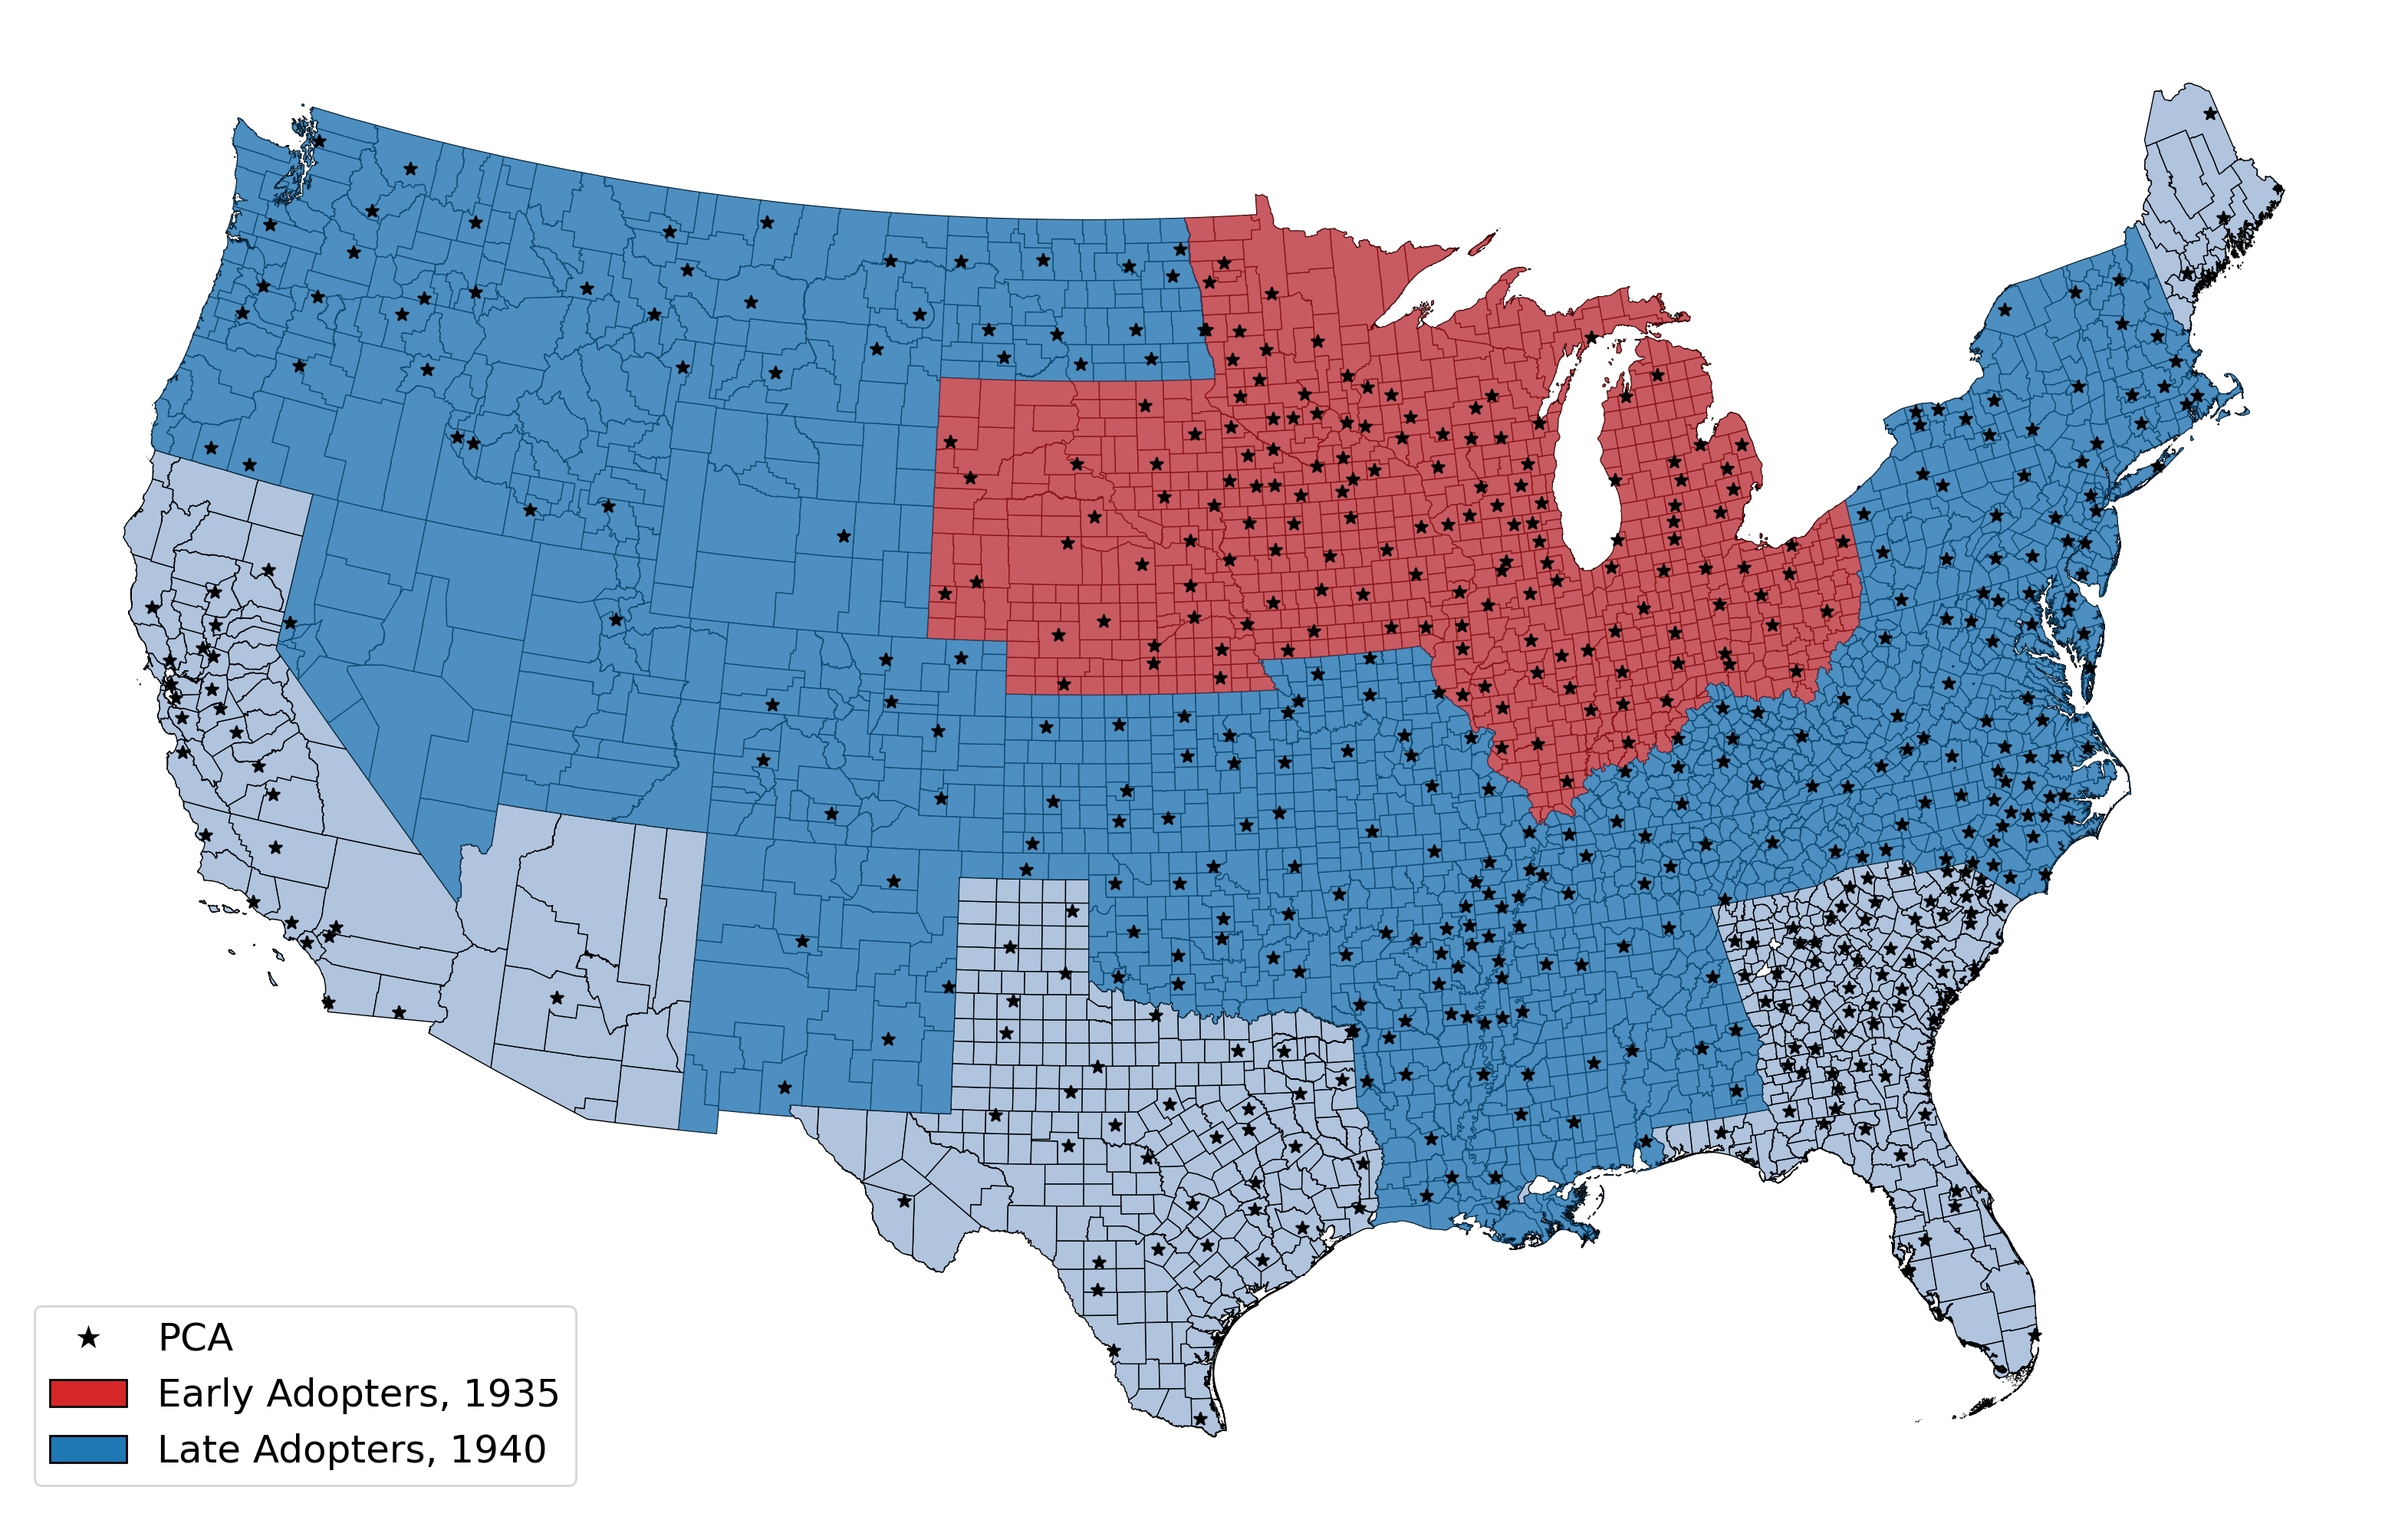
\includegraphics[width=\textwidth]{corn_map.png}

Early adopters have non-zero adoption rates in 1935, late adopters in 1940.
\end{figure}

\begin{table}[!htbp] \centering 
    \caption{Corn Yield and State Hybrid Adoption} 
    \label{hybrid_table} 
    \begin{threeparttable}[t]
\footnotesize
\begin{tabular}{@{\extracolsep{5pt}}lcccc} 
\\[-1.8ex]\hline 
\hline\\[-1.8ex] & \multicolumn{4}{c}{Corn Yield}  \\
\cline{2-5} 
\\ Distance from PCA & All States & Early Adopters & Late Adopters & Never Adopters \\ 
\hline \\[-1.8ex] 
\\\multicolumn{1}{l}{\textbf{1935}} & & & & \\ 
$(30, 45]$ km    & $-$0.054$^{**}$     & $-$0.070      & $-$0.034         & $-$0.006 \\
                 & (0.025)             & (0.043)       & (0.036)          & (0.065) \\
                 &                     &               &                  & \\
$(45, 60]$ km    & $-$0.068$^{**}$     & $-$0.037      & $-$0.083$^{**}$  & $-$0.058 \\
                 & (0.030)             & (0.057)       & (0.040)          & (0.073) \\
                 &                     &               &                  & \\
$(60, 100]$ km   & $-$0.089$^{***}$    & $-$0.047      & $-$0.092$^{**}$  & $-$0.055 \\
                 & (0.032)             & (0.061)       & (0.045)          & (0.078) \\
                 &                     &               &                  & \\
$>$ 100 km       & $-$0.120$^{*}$      & $-$0.222      & $-$0.058         & $-$0.088 \\
                 & (0.062)             & (0.153)       & (0.088)          & (0.126) \\
% \hline \\[-1.8ex]     
% Observations                       & 13,929              & 3,852         & 7,424            & 2,653 \\
% Adjusted R$^{2}$                   & 0.786               & 0.871         & 0.765            & 0.610 \\
% Pre-Trend F-test                   & 0.941               & 1.202         & 1.609            & 0.748 \\
% Pre-Trend P-Value                  & 0.481               & 0.294         & 0.117            & 0.649 \\
% \hline 
% \hline \\[-1.8ex] 
\\\multicolumn{1}{l}{\textbf{1940}} & & & & \\ 


% \\Distance from PCA & All States & Early Adopters & Late Adopters & Never Adopters \\ 
% \hline \\[-1.8ex] 
$(30, 45]$ km                      & $-$0.031       & 0.014          & $-$0.068       & 0.010 \\
                                   & (0.029)        & (0.025)        & (0.043)        & (0.094) \\
                                   &                &                &                & \\
$(45, 60]$ km                      & $-$0.010       & 0.001          & $-$0.017       & 0.0002 \\
                                   & (0.035)        & (0.039)        & (0.051)        & (0.107) \\
                                   &                &                &                & \\
$(60, 100]$ km                     & $-$0.089$^{**}$& $-$0.033       & $-$0.100$^{**}$& $-$0.099 \\
                                   & (0.035)        & (0.042)        & (0.050)        & (0.108) \\
                                   &                &                &                & \\
$>$ 100 km                         & $-$0.137$^{**}$& $-$0.256$^{**}$& $-$0.108       & $-$0.063 \\
                                   & (0.062)        & (0.123)        & (0.090)        & (0.139) \\
                                   &                &                &                & \\
\hline \\[-1.8ex]               
Observations                       & 13,929         & 3,852          & 7,424          & 2,653 \\
Adjusted R$^{2}$                   & 0.786          & 0.871          & 0.765          & 0.610 \\
Pre-Trend F-test                   & 0.941          & 1.202          & 1.609          & 0.748 \\
Pre-Trend P-Value                  & 0.481          & 0.294          & 0.117          & 0.649 \\
\hline 
\hline \\[-1.8ex] 
\end{tabular}
\begin{tablenotes}
    \item {\footnotesize * \(p<0.10\), ** \(p<0.05\), *** \(p<0.01\).}
    \item {\footnotesize All specifications include county, year, and state-by-year fixed effects.}
  \end{tablenotes}
\end{threeparttable} 
\end{table} 



\end{appendices}
\newpage
\bibliography{references}
\bibliographystyle{chicago}

\end{document}